% !TEX root = task-1-15-8.tex
% Editable task bank. Append new BankTask blocks at the end of the document.
\documentclass[12pt,a4paper]{article}
\usepackage{physics-textbook}
\usepackage{graphicx,needspace}
\usetikzlibrary{decorations.pathmorphing}
\newif\ifShowSolutions
\ifdefined\TutorEdition
  \ShowSolutionstrue
\else
  \ShowSolutionsfalse % Change to \ShowSolutionstrue to display solutions.
\fi
\newcounter{banktask}
\newsavebox{\BankTaskBox}
\newcommand{\BankTaskContent}[3]{%
  \noindent\textbf{\thebanktask.}\quad #2\par
  \ifShowSolutions
    \Needspace{50mm}% Keep the solution heading with its opening text or diagram.
    #3\par
    \ifdefined\TutorEdition
      \ifcsname TutorSource#1\endcsname
        \nopagebreak\smallskip{\small\csname TutorSource#1\endcsname\par}%
      \fi
    \fi
  \fi
}
\newcommand{\BankTask}[3]{%
  \refstepcounter{banktask}\par\medskip
  \sbox{\BankTaskBox}{\begin{minipage}{\linewidth}%
    \BankTaskContent{#1}{#2}{#3}\end{minipage}}%
  \ifdim\dimexpr\ht\BankTaskBox+\dp\BankTaskBox\relax>\dimexpr\textheight-20mm\relax
    \Needspace{35mm}\BankTaskContent{#1}{#2}{#3}%
  \else
    \Needspace{\dimexpr\ht\BankTaskBox+\dp\BankTaskBox\relax}%
    \noindent\usebox{\BankTaskBox}\par
  \fi
  \medskip
}
\begin{document}
\BookSubsection{1.15.8}{Закон изменения механической энергии}


% Source sdamgia-7175: https://phys-ege.sdamgia.ru/problem?id=7175
\BankTask{sdamgia-7175}{
Шарик массой $200\,\text{г}$ падает с высоты $20\,\text{м}$ с начальной скоростью, равной нулю. Какова его кинетическая энергия в момент перед ударом о землю, если потеря энергии за счёт сопротивления воздуха составила $4\,\text{Дж}$? Ускорение свободного падения принять равным $10\,\text{м/с}^2$.
}{
\smallskip\noindent\textbf{Решение}\par
В верхней точке кинетическая энергия шарика равна нулю, так как начальная скорость равна нулю. Тогда полная энергия шарика равна его потенциальной энергии в верхней точке $E_p=m \cdot g \cdot h=0{,}2\,\text{кг} \cdot 10 \frac{\text{м}}{\text{с} ^{2}} \cdot 20\,\text{м}=40\,\text{Дж}.$ 

Согласно закону сохранения энергии, $E_1=E_{\text{к}} + \delta E,$ где $E_{k}$ — это кинетическая энергия шарика перед ударом об землю, а $\delta E$ — потеря энергии за счет сопротивления воздуха. Тогда $E_k=E_1 - \delta E=40 - 4=36\,\text{Дж}.$

Ответ: $36$.
}

% Source sdamgia-9495: https://phys-ege.sdamgia.ru/problem?id=9495
\BankTask{sdamgia-9495}{
Изначально покоившееся тело массой $2\,\text{кг}$ начинает соскальзывать с наклонной плоскости. За некоторый промежуток времени сила тяжести совершает над телом механическую работу $10\,\text{Дж}$, при этом выделяется количество теплоты $1\,\text{Дж}$. Определите модуль импульса, который в результате этого приобретает тело.
}{
\smallskip\noindent\textbf{Решение}\par
При условии, что изначально тело покоилось, работа силы тяжести пойдет на увеличение кинетической энергии тела и нагрев: 

\[A=E_{\text{к}} + Q= \frac{p ^{2}}{2m} + Q.\]

Найдем отсюда величину приобретенного модуля импульса:

\[p= \sqrt{2m ( A - Q )} = \sqrt{2 \cdot 2 \cdot 9} =6\,\text{кг} \cdot \text{м}/\text{с}.\]

Ответ: $6\,\text{кг}\cdot\text{м/с}$.
}

% Source sdamgia-9730: https://phys-ege.sdamgia.ru/problem?id=9730
\BankTask{sdamgia-9730}{
Телу массой $4\,\text{кг}$, находящемуся на шероховатой горизонтальной плоскости, сообщили вдоль неё скорость $10\,\text{м/с}$. Определите модуль работы, совершённой силой трения, с момента начала движения тела до того момента, когда скорость тела уменьшится в $2$ раза.
}{
\smallskip\noindent\textbf{Решение}\par
Работа силы трения идет на уменьшение кинетической энергии тела. Запишем закон сохранения энергии:

\[A=E_{\text{кин}1} - E_{\text{кин}2}= \frac{mV_1 ^{2}}{2} - \frac{mV_2 ^{2}}{2} = \frac{3mV_1 ^{2}}{8} = \frac{3 \cdot 4 \cdot 100}{8} =150\,\text{Дж}.\]

Ответ: $150$.
}

% Source sdamgia-51008: https://phys-ege.sdamgia.ru/problem?id=51008
\BankTask{sdamgia-51008}{
Шарик массой $400\,\text{г}$ падает с некоторой высоты. Начальная скорость шарика равна нулю. Его кинетическая энергия при падении на землю равна $7\,\text{Дж}$, а потеря энергии за счёт сопротивления воздуха составила $1\,\text{Дж}$. С какой высоты упал шарик?
}{
\smallskip\noindent\textbf{Решение}\par
Работа силы сопротивления $A_{\text{сопр}}=E_{\text{полн}2} - E_{\text{полн}1},$ где $E_{\text{полн}1}=mgh,$ $E_{\text{полн}2}=E_{\text{к}2}.$ Тогда высота, с которой упало тело, с учетом, что работа сопротивления отрицательна, равна

\[h= \frac{E_{\text{к}2} + |A_{\text{сопр}}|}{mg} = \frac{1 + 7}{0{,}4 \cdot 10} =2\,\text{м}.\]

Ответ: $2$.
}

% Source sdamgia-11260: https://phys-ege.sdamgia.ru/problem?id=11260
\BankTask{sdamgia-11260}{
У основания шероховатой наклонной плоскости покоится маленькая шайба массой $100\,\text{г}$. Шайбе сообщают импульс $0{,}6\,\text{кг}\cdot\text{м/с}$ в направлении вверх вдоль наклонной плоскости. После этого шайба поднимается по плоскости и останавливается на высоте $20\,\text{см}$ от основания. Какое количество теплоты выделяется при движении шайбы?
}{
\smallskip\noindent\textbf{Решение}\par
По закону сохранения энергии, приобретенная кинетическая энергия шайбы пойдет на изменение ее потенциальной энергии и на выделение тепла при движении по шероховатой поверхности. Отсюда тепло, которое выделится при движении, равно:

\[Q= \frac{p ^{2}}{2m} - mgh= \frac{0{,}36}{0{,}2} - 0{,}1 \cdot 10 \cdot 0{,}2=1{,}6\,\text{Дж}.\]

Ответ: $1{,}6$.
}

% Source sdamgia-7780: https://phys-ege.sdamgia.ru/problem?id=7780
\BankTask{sdamgia-7780}{
Человек стоит на гладком льду и держит в руках снежок. Масса снежка в $50$ раз меньше массы человека. При горизонтальном бросании снежка человек совершил работу $76{,}5\,\text{Дж}$. Какова кинетическая энергия снежка после броска?
}{
\smallskip\noindent\textbf{Решение}\par
Пусть масса человека $m.$ По закону сохранения импульса импульсы снежка и человека после броска равны:

\[p_{\text{ч}} = p_{\text{с}} \Longleftrightarrow m v _{\text{ч}} = m/50 \cdot v _{\text{с}} \Longleftrightarrow v _{\text{с}} = 50 v _{\text{ч}}.\]

Выразим кинетическую энергию снежка через кинетическую энергию человека: 

\[E_{\text{кс}} = \frac{m/50 \cdot ( v _{\text{с}} ) ^{2}}{2} = \frac{m/50 \cdot ( 50 v _{\text{ч}} ) ^{2}}{2} =50 \frac{m v _{\text{ч}} ^{2}}{2} = 50E_{\text{кч}}.\]

То есть $E_{\text{кч}} = E_{\text{кс}}/50.$

Суммарная кинетическая энергия снежка и человека равна работе, совершенной человеком:

\[A = E_{\text{кч}} + E_{\text{кс}} \Longleftrightarrow A = ( \frac{1}{50} + 1 ) E_{\text{кс}}\Longleftrightarrow E_{\text{кс}} = \frac{50}{51} A,\]

откуда кинетическая энергия снежка:

\[E_{\text{кс}} = \frac{50 \cdot 76{,}5\,\text{Дж}}{51} = 75\,\text{Дж}.\]

Ответ: $75$.
}

% Source sdamgia-6917: https://phys-ege.sdamgia.ru/problem?id=6917
\BankTask{sdamgia-6917}{
Тела $1$ и $2$ взаимодействуют только друг с другом. Изменение кинетической энергии тела $2$ за некоторый промежуток времени равно $10\,\text{Дж}$. Работа, которую совершили за этот же промежуток времени силы взаимодействия тел $1$ и $2$, равна $30\,\text{Дж}$. Чему равно изменение кинетической энергии тела $1$ за это время?
}{
\smallskip\noindent\textbf{Решение}\par
Поскольку тела $1$ и $2$ взаимодействуют только друг с другом, они образуют замкнутую систему.

Кинетической энергией системы называют сумму кинетических энергий всех тел, входящих в систему. $E_{\text{к}}=E_{\text{к}1} + E_{\text{к}2},$ а изменение кинетической энергии $\delta E_{\text{к}}= \delta E_{\text{к}1} + \delta E_{\text{к}2}.$

Изменение кинетической энергии системы равно работе всех внутренних сил. Таким образом, получаем: 

\[\delta E_{\text{к}1}= \delta E_{\text{к}} - \delta E_{\text{к}2}=A - \delta E_{\text{к}2}=30\,\text{Дж} - 10\,\text{Дж}=20\,\text{Дж}.\]

Ответ: $20$.
}

% Source sdamgia-2946: https://phys-ege.sdamgia.ru/problem?id=2946
\BankTask{sdamgia-2946}{
Кусок пластилина сталкивается со скользящим навстречу по горизонтальной поверхности стола бруском и прилипает к нему. Скорости пластилина и бруска перед ударом направлены взаимно противоположно и равны $v_{\text{пл}}=15\,\text{м/с}$ и $v_{\text{бр}}=5\,\text{м/с}$. Масса бруска в $4$ раза больше массы пластилина. К моменту, когда скорость слипшихся бруска и пластилина уменьшилась в $2$ раза, они переместились на $0{,}22\,\text{м}$. Определите коэффициент трения $\mu$ бруска о поверхность стола.
}{
\smallskip\noindent\textbf{Решение}\par
Пусть $m$ — масса куска пластилина, $M$ — масса бруска, $v _0$ — начальная скорость бруска с пластилином после взаимодействия. Согласно закону сохранения импульса: $M v _{\text{бр}} - m v _{\text{пл}}= ( M + m ) v _0.$

Так как $M=4m$ и $v _{\text{бр}}= \frac{1}{3} v _{\text{пл}},$ то $4m \frac{1}{3} v _{\text{пл}} - m v _{\text{пл}}=5m v _0$ и $v _0= \frac{1}{15} v _{\text{пл}}.$

По условию конечная скорость бруска с пластилином $v =0{,}5 v _0.$

По закону сохранения и изменения механической энергии: 

\[\frac{( M + m ) v _0 ^{2}}{2} = \frac{( M + m ) v ^{2}}{2} + \mu ( M + m ) gS,\]

 откуда: 

\[\frac{5m(\frac1{15}v_{\text{пл}})^2}{2}=\frac{5m(0{,}5\frac1{15}v_{\text{пл}})^2}{2}+5m\mu gS,\]

$\frac{1}{2 \cdot 15 ^{2}} \cdot v _{\text{пл}} ^{2} - \frac{0{,}25}{2 \cdot 15 ^{2}} \cdot v _{\text{пл}} ^{2} =\mu gS$ и $\mu = \frac{3}{8 \cdot 15 ^{2}} \cdot \frac{v _{\text{пл}} ^{2}}{Sg} = \frac{3 \cdot 15 ^{2}}{8 \cdot 15 ^{2} \cdot 0{,}22 \cdot 10} \approx 0{,}17.$

Ответ: $\mu =0{,}17.$
}

% Source sdamgia-10238: https://phys-ege.sdamgia.ru/problem?id=10238
\BankTask{sdamgia-10238}{
На горизонтальном гладком столе лежит длинная доска массой $M=10\,\text{кг}$, а на её левом конце --- деревянный брусок массой $m=1\,\text{кг}$ (см. рисунок). В брусок попадает и прилипает к нему пластилиновый снаряд массой $m_0=200\,\text{г}$, летевший горизонтально по направлению вдоль доски со скоростью $V_0=10\,\text{м/с}$, после чего брусок скользит до остановки по шероховатой доске, не сваливаясь с неё. Какое количество теплоты $Q$ выделится в этой системе в течение всего процесса?\begin{center}\begin{tikzpicture}[book diagram]
\draw(-.5,0)--(5,0);\draw[book body](.3,.08)rectangle(4.8,.32);\draw[book body](.5,.32)rectangle(1.3,.9);
\node[above]at(.9,.9){$m$};\node[above]at(3,.32){$M$};\node[left]at(-.15,.22){$\mu$};\draw[->](-.05,.22)--(.7,.32);\draw[->](-.6,.6)--(.4,.6)node[midway,above]{$V_0$};\fill(-.6,.6)circle(.07)node[left]{$m_0$};
\end{tikzpicture}\end{center}
}{
\smallskip\noindent\textbf{Решение}\par
$1$. На всю систему «пуля + брусок + доска» по горизонтали не действуют внешние силы, поэтому справедлив закон сохранения проекции импульса по этому направлению: $m_0V_0= ( m_0 + m + M ) V,$ где $V$ — скорость движения системы после остановки бруска. Таким образом,

\[V= \frac{m_0V_0}{m_0 + m + M} .\]

$2$. В начальном состоянии механическая энергия системы равна кинетической энергии пули $E_{\text{к}1}= \frac{m_0V_0 ^{2}}{2} ,$ а в конечном — кинетической энергии системы $E_{\text{к}2}= \frac{( m_0 + m + M ) V ^{2}}{2} = \frac{m_0 ^{2} V_0 ^{2}}{2 ( m_0 + m + M )} .$

$3$. По закону изменения механической энергии разность этих кинетических энергий выделяется в виде теплоты:

\[Q=E_{\text{к}1} - E_{\text{к}2}= \frac{m_0V_0 ^{2}}{2} \cdot \frac{m + M}{m_0 + m + M} \approx9{,}8\,\text{Дж}.\]

Ответ: $Q= \frac{m_0V_0 ^{2}}{2} \cdot \frac{m + M}{m_0 + m + M} \approx9{,}8\,\text{Дж}.$
}

% Source sdamgia-37576: https://phys-ege.sdamgia.ru/problem?id=37576
\BankTask{sdamgia-37576}{
У нижнего края наклонной плоскости, составляющей с горизонтом угол $\alpha=30^\circ$, находится небольшой брусок. В некоторый момент ему сообщают начальную скорость $v_0=4\,\text{м/с}$, направленную вверх вдоль плоскости. Коэффициент трения бруска о плоскость равен $\mu=0{,}3$. После подъёма по прямой на максимально возможную высоту брусок соскальзывает вниз. Найдите скорость $v_{\text{к}}$ бруска в момент его возврата в исходную точку.
}{
\smallskip\noindent\textbf{Решение}\par
$1$. На первом этапе брусок движется вверх равнозамедленно с начальной скоростью $v _0$ и проходит до остановки путь $s$, а на втором этапе брусок движется равноускоренно без начальной скорости и проходит тот же путь $s$, ускоряясь до конечной скорости $v _{\text{к}} = at,$ где $a$ и $t$ — модуль ускорения при движении вниз и время этого движения.

\begin{center}\begin{tikzpicture}[book diagram,scale=.9]
\draw(0,0)--(5,0);\foreach \x in{0,.2,...,5}{\draw(\x,0)--++(-.13,-.14);}
\draw[book body](0,0)--(4.8,3.49);\draw(.7,0)arc(0:36:.7);\node at(.95,.27){$\alpha$};
\coordinate(C)at(2.891,2.33);
\begin{scope}[shift={(C)},rotate=36]\draw[book body,fill=orange!30](-.42,-.185)rectangle(.42,.185);\end{scope}
\draw[->,thick](C)--++(126:1.25)node[above left]{$\vec N$};
\draw[->,thick](C)--++(36:1.3)node[above right]{$\vec F_{\text{тр}}$};
\draw[->,thick](C)--++(-90:1.35)node[below right]{$m\vec g$};
\draw[->,thick](2.7,1.96)--++(216:1.1)node[above left]{$\vec v$};
\node at(4,1.7){$\mu$};\draw[->](3.85,1.5)..controls(3.4,1.2)and(3.5,1.8)..(3.55,2.1);
\draw[->](.8,2.8)--(.8,2.05)node[left,midway]{$\vec g$};
\end{tikzpicture}\end{center}

$2$. На брусок при его движении по наклонной плоскости вниз действуют сила тяжести $mg$, направленная вниз, сила нормальной реакции $N$, перпендикулярная плоскости, и сила трения скольжения $F_{\text{тр}} = \mu N$ (закон Амонтона-Кулона), направленная вдоль плоскости противоположно скорости бруска (см. рис.).

$3$. Записывая второй закон Ньютона в проекциях на направления вдоль плоскости и перпендикулярно ей, получаем, что:

$N=mg \cos \alpha ,$ $ma=mg \sin \alpha - \mu N,$ откуда $a=g ( \sin \alpha - \mu \cos \alpha ) .$

$4$. Поскольку на втором этапе выполняются кинематические соотношения:

$t= \frac{v _{\text{к}}}{a}$ и $s= \frac{at ^{2}}{2} ,$ то $s= \frac{v ^{2} _{\text{к}}}{2a} .$

$5$. Так как потенциальная энергия бруска в начале и в конце движения одинакова, то из закона изменения механической энергии получаем:

\[\frac{m v _0 ^{2}}{2} = \frac{m v _{\text{к}} ^{2}}{2} + \mu mg \cos \alpha \cdot 2s.\]

Подставляя выражения для $S$ и $a$, получаем, что:

\[v _0 ^{2} = v ^{2} _{\text{к}} ( 1 + \frac{2\mu \cos \alpha}{\sin \alpha - \mu \cos \alpha} ) = v ^{2} _{\text{к}} \frac{\tan \alpha + \mu}{\tan \alpha - \mu} ,\]

 откуда:

\[v _{\text{к}}= v _0 \sqrt{\frac{\tan \alpha - \mu}{\tan \alpha + \mu}} .\]

$6$. Подставляя данные из условия, получаем:

\[v _{\text{к}}\approx 4 \cdot \sqrt{\frac{0{,}577 - 0{,}3}{0{,}577 + 0{,}3}} \approx 2{,}25\,\text{м}/\text{с}.\]

Ответ: $v _{\text{к}}\approx 2{,}25\,\text{м}/\text{с}.$
}


% Source E9E545: https://ege.fipi.ru/bank/questions.php?search=1&proj=BA1F39653304A5B041B656915DC36B38&qid=E9E545
\BankTask{E9E545}{
Шарик массой $100\,\text{г}$ падает с некоторой высоты. Начальная скорость шарика равна нулю. Его кинетическая энергия при падении на землю равна $6\,\text{Дж}$, а потеря энергии за счёт сопротивления воздуха составила $1\,\text{Дж}$. С какой высоты упал шарик? Выразите ответ в метрах.
}{
\smallskip\noindent\textbf{Решение от GPT}\par
$m=0{,}1\,\text{кг}$. При $g=10\,\text{м}/\text{с}^2$ начальная энергия $mgh=E_{\text{к}}+E_{\text{потерь}}$, откуда $h=(6+1)/(0{,}1\cdot10)=7\,\text{м}$. Ответ: $7\,\text{м}$.
}

% Source 2785A3: https://ege.fipi.ru/bank/questions.php?search=1&proj=BA1F39653304A5B041B656915DC36B38&qid=2785A3
\BankTask{2785A3}{
Мальчик на санках спустился с ледяной горы высотой $10\,\text{м}$ и проехал по горизонтали до остановки $50\,\text{м}$. Чему равен коэффициент трения санок по горизонтальной поверхности? Считать, что по склону горы санки скользили без трения.
}{
\smallskip\noindent\textbf{Решение от GPT}\par
На склоне $E_{\text{к}}=mgh$, на горизонтальном участке $\mu mgs=mgh$. Поэтому $\mu=h/s=10/50=0{,}2$.
}

% Source E74C4C: https://ege.fipi.ru/bank/questions.php?search=1&proj=BA1F39653304A5B041B656915DC36B38&qid=E74C4C
\BankTask{E74C4C}{
Учащиеся роняли с башни шарики для настольного тенниса и снимали их полёт цифровой видеокамерой. Обработка видеозаписей позволила построить графики зависимости пути $s$, пройденного шариком, и его скорости $v$ от времени падения $t$.
\begin{center}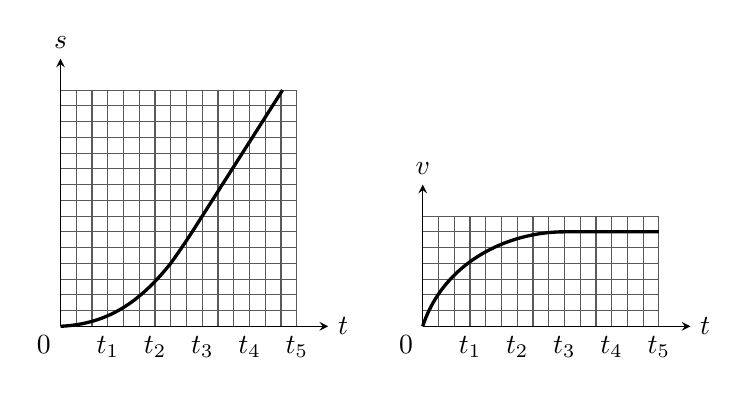
\begin{tikzpicture}[x=.2cm,y=.2cm,>=stealth]
\draw[thin,black!65,step=1] (0,0) grid (15,15);
\draw[->] (0,0)--(17,0) node[right] {$t$};\draw[->] (0,0)--(0,17) node[above] {$s$};
\node[below left] at (0,0) {$0$};
\foreach \x/\i in {3/1,6/2,9/3,12/4,15/5} \node[below] at (\x,0) {$t_{\i}$};
\draw[very thick] (0,0) .. controls (3,.15) and (5,1.5) .. (7,4) .. controls (8,5.4) and (8.49,6.2) .. (9,7) --(14.1,15);
\begin{scope}[xshift=4.6cm]
\draw[thin,black!65,step=1] (0,0) grid (15,7);
\draw[->] (0,0)--(17,0) node[right] {$t$};\draw[->] (0,0)--(0,9) node[above] {$v$};
\node[below left] at (0,0) {$0$};
\foreach \x/\i in {3/1,6/2,9/3,12/4,15/5} \node[below] at (\x,0) {$t_{\i}$};
\draw[very thick] (0,0) .. controls (1.3,4) and (5.3,6) .. (9,6) --(15,6);
\end{scope}\end{tikzpicture}\end{center}
\begin{enumerate}
\item В течение всего времени падения ($0$ — $t_{5}$) потенциальная энергия шарика в поле тяжести, отсчитываемая от основания башни, уменьшалась.
\item В течение всего времени падения ($0$ — $t_{5}$) величина импульса шарика постоянно возрастала.
\item Величина ускорения, с которым падал шарик, уменьшалась в интервале времени ($0$ — $t_{3}$).
\item Величина ускорения, с которым падал шарик, увеличивалась в интервале времени ($0$ — $t_{3}$) и оставалась постоянной при $t>t_{4}$.
\item Сумма кинетической и потенциальной энергий шарика оставалась неизменной во время падения.
\end{enumerate}
}{
\smallskip\noindent\textbf{Решение от GPT}\par
Шарик всё время опускается: $E_{\text{п}}=mgh$ уменьшается. Наклон графика $v(t)$ до $t_3$ уменьшается, значит ускорение уменьшается. Затем скорость и импульс постоянны. Сопротивление воздуха совершает отрицательную работу, поэтому механическая энергия не сохраняется. Ответ: $13$.
}

% Source 25952: https://phys-ege.sdamgia.ru/problem?id=25952
\BankTask{25952}{
\begin{center}\begin{tikzpicture}[task graph,>=stealth]\draw (0,0)--(3,0)--(4.8,2.5)--(1.8,2.5)--cycle (4.8,2.5)--(4.8,1.1)--(3,0);\draw (3.55,.34) arc (32:54:.65) node[midway,right]{\(\alpha\)};\draw[fill=gray!15](2.04,1.13)arc(180:360:.25 and .085)--(2.54,1.30)arc(0:180:.25 and .085)--cycle;\draw(2.04,1.30)arc(180:360:.25 and .085);\draw[->] (2.29,1.21)--(3.3,1.21) node[above]{\(\vec F\)};\end{tikzpicture}\end{center}На рисунке изображена плоскость, наклоненная под углом $\alpha =30 ^\circ$ к горизонту и тело, находящееся на ней. Если к телу приложить силу $F=1{,}7\,\text{Н},$ как показано на рисунке, то тело начнет скользить. Масса тела равна $500\,\text{г}$. Определите коэффициент трения тела о поверхность.
Какие законы Вы используете для описания движения шайбы? Обоснуйте их применение к данному случаю.
}{
\smallskip\noindent\textbf{Решение}\par
Обоснование. Систему отсчета, связанную с неподвижной плоскостью, можем считать инерциальной. Движение шайбы поступательное. Следовательно, ее можно считать материальной точкой. При движении шайбы по наклонной поверхности на него действуют силы тяжести, приложенная сила, трения и реакции опоры. В ИСО при движении тела применим второй закон Ньютона.

Перейдем к решению. На тело действуют силы:F, $F_{\,\text{тр}},$ N, $mg.$ Выберем оси координат: $\,\text{Ох}$  — вдоль нижней грани, $\,\text{О}y$  — вверх по наклонной плоскости, $\,\text{О}z$  — перпендикулярно к оси $\,\text{О}y.$ Брусок движется равномерно. Следовательно, по второму закону Ньютона: 
\begin{center}\begin{tikzpicture}[task graph,>=stealth]\draw (0,0)--(3,0)--(4.8,2.5)--(1.8,2.5)--cycle (4.8,2.5)--(4.8,1.1)--(3,0);\draw (3.55,.34) arc (32:54:.65) node[midway,right]{\(\alpha\)};\draw[fill=gray!15](2.04,1.13)arc(180:360:.25 and .085)--(2.54,1.30)arc(0:180:.25 and .085)--cycle;\draw(2.04,1.30)arc(180:360:.25 and .085);\draw[->] (2.29,1.21)--(3.3,1.21) node[above]{\(\vec F\)};\draw[->] (2.29,1.21)--(2.29,.28) node[right]{\(m\vec g\)};\draw[->] (2.29,1.21)--(1.81,2.05) node[above]{\(\vec N\)};\draw[->] (2.29,1.21)--(1.33,1.55) node[below]{\(\vec F_{\text{тр}}\)};\draw[->] (-.6,0)--(5.25,0) node[below]{\(x\)};\draw[->] (-.45,-.63)--(2.45,3.42) node[above]{\(y\)};\draw[->] (.29,-.61)--(-1.22,2.57) node[left]{\(z\)};\end{tikzpicture}\end{center}

\[\overrightarrow{F} + m\vec g + \vec N + \vec F_{\,\text{тр}}=0.\]
 
Найдем проекции на координатные оси:

\[\begin{aligned} Ox:&\quad F-F_{\text{тр},x}=0,\\Oy:&\quad F_{\text{тр},y}-mg\sin\alpha=0,\\Oz:&\quad N-mg\cos\alpha=0.\end{aligned}\]

Учитывая, что $F_{\,\text{тр}}=\mu N$ и $F_{\,\text{тр}}= \sqrt{F_{\text{тр},x}^{2}+F_{\text{тр},y}^{2}} ,$ получаем: $( \mu m g ) ^2 \cos ^2 \alpha =F ^2 + ( mg ) ^2 \sin ^2 \alpha .$

Выразим коэффициент трения:

\[\mu= \frac{\sqrt{F ^2 + ( mg \sin \alpha ) ^2}}{mg \cos \alpha} = \frac{\sqrt{1{,}7 ^2 + ( 0{,}5 \cdot 10 \cdot 0{,}5 ) ^2}}{0{,}5 \cdot 10 \cdot \cos 30 ^\circ} \approx 0{,}7.\]

Ответ: $0{,}7$.
}

\end{document}
